\cotefile{42}
\scanpage{2}
\uline{Réseau\unsure{’|} d'anneaux locaux}

est formé d'un ensemble ordonné $X$, et \deleted{pour \unsure{tout|tt} $x\in X$, d} d'un système in\uline{du}ctif d'anneaux locaux $(O_x)_{x\in X}$, [donc si $x\leq y$, on a $O_x\to O_y$) tel que pour $x\leq y$, $O_x\to O_y$ induise un isomorphisme $(\underline{O}_x)_{p_{xy}}\to\underline{O}_y$, (où $p_{xy}$ est l'image \unsure{inverse|réciproque} de $\unsure{r|\mathfrak{r}|\mathfrak{m}}(\underline{O}_y)$) et que \deleted{$p_{xy}\unsure{\supset|\supseteq}p_{xy'}\Rightarrow y\unsure{\leq|\geq}y'$} \inserted{l'on obtienne ainsi une correspondance biunivoque entre les $y\geq x$ et les idéaux premiers de $O_x$}.
% slanted
\margin{Notation $X,Y$ pour des réseaux.}

Un hom. d'un réseau $X$ dans un autre $Y$ : hom des systèmes inductifs d'anneaux \uline{locaux}, i.e. \unsure{formé} d'une application \deleted{\unsure{continue}} croissante $X\xrightarrow{f}Y$, et pour \unsure{tt|tout} $x\in X$ d'un hom \uline{local} $\underline{O}_{f(x)}\to\underline{O}_x$, compatible avec les applications de \deleted{\unsure{spécialisati|spécialisation}} générisation.

Soit $\unsure{\mathcal R|\mathscr R|R}$ la catégorie des réseaux, $\unsure{S|\mathcal S}$ la catégorie des préschémas. On a un foncteur canonique $S\xrightarrow{\unsure{\rho|P|p}}\mathcal R$.

Réseau sur un autre, sur un préschéma.

Soit $S$ un préschéma \unsure{loc|loc.} noethérien,
% archive sheet number: 1
\scanpage{3}
soient $\underline{\unsure{S|\mathcal S}}/S$ et $\underline{\unsure{\mathcal R|\mathscr R|R}}/S$ les catégories des préschémas (\unsure{resp$^{\mathrm{t}}$|respt.} réseaux) sur $S$, $\underline{S}_0/S$ la \unsure{ss-catégorie|ss. catégorie} de $\underline{S}/S$ formée des \inserted{$S$-}préschémas loc. de type fini. Alors \deleted{\unsure{$\rho$ :|$p$}}
\[
\unsure{\rho|P|p}:\underline{S}_0/S\longrightarrow\underline{\mathcal R}/S
\]
est \uline{pleinement fidèle}\unsure{,|.}
\deleted{En effet, un hom \deleted{\unsure{appl|eff}} de réseaux $\rho(X)\longrightarrow\rho(Y)$ est continu pour les topologies sous-jacentes, car on est ramené au cas où $X$ est affine donc noethérien, \unsure{donc|alors} les pts de $X$ sont spécialisations d'un \unsure{nb|nbre|ens.} fini d'entre eux, donc les pts de $=$ les pts de $f(X)$ \unsure{- - - -}.}
% slanted
\margin{est-il inutile de mettre des conditions de finitude sur $\unsure{Y|S}$ ??}

\deleted{Plus généralement, si $Y$ est \inserted{\unsure{loc|loc.}} de type fini sur $S$, \deleted{\unsure{des préschémas|deux préschémas}} \inserted{$X$ quelconque}, alors}
\[
\deleted{\operatorname{Hom}_{S}(X,Y)\xrightarrow{\sim}H_{S}(\rho(X),\rho(Y))}
\]
\deleted{[bijectif]. En effet, \inserted{$f\in\operatorname{Hom}_{S}\unsure{(|}\rho(X),\rho(Y))$. (\unsure{évidemt|d'ailleurs} \unsure{tjs|tjrs} \uline{inj}.} soit $x\in X$, $y=f(x)$, considérons $\underline{O}_y\to\underline{O}_x$, il définit un hom d'un voisinage \inserted{\deleted{\unsure{ouvert}}} $U$ de $x$ dans un voisinage \unsure{ouvert} $V$ de $y$.}
% archive sheet number: 2
\scanpage{4}
\uline{Proposition} Soit $X$ un espace loc. noeth. dont toute partie fermée irréductible a exactement un point générique. \deleted{Soit} $F$ un faisceau sur $X$, satisfaisant la condition suivante : pour tt $x\in X$, il existe un \deleted{partie} \inserted{voisinage} ouvert \deleted{non vide} $U$ de $\overset{\deleted{\text{--}}}{x}$ tel que pour \unsure{ts|tt} $y\in\bar{x}\cap U$, l'application naturelle $F_y\to F_x$ soit \uline{injective}. \deleted{Alors}

\deleted{Soit} Ordonnons $X$ par $y\unsure{\leq|\leqq}x\Leftrightarrow\bar{y}\supset\bar{x}$ i.e. $\bar{y}\ni x$, soit $\widetilde F$ le \deleted{faisceau} système \deleted{inductif} \inserted{projectif} sur $X$ défini par $F$, considérons l'application naturelle
\[
\Gamma(X,F)\unsure{\text{---}|\longrightarrow}\varprojlim\widetilde F
\]
Cette application est \uline{bijective}.

La question est locale. On peut donc supposer $X$ noethérien. \deleted{Soit $U$ un ouvert de} \inserted{Il suffit de prouver} que $\longrightarrow$ est surjective, soit $(\xi_x)_{x\in X}\in\varprojlim F$.

\uline{Lemme 1} Soit $s$ une section de $F$ sur $U$. Alors l'ens des pts $x\in U$ tels que $s_x=\xi_x$ est \uline{ouvert}.

S'il contient $x$, il contient les $y\leq x$ i.e. \unsure{tels que|les pour} $\bar{y}\ni x$, il suffit de montrer qu'il est \uline{constructible}, donc que s'il contient $x$, il contient \deleted{\unsure{les|le}} un ouvert non vide de $\bar{x}$. Or il existe un ouvert non vide $U$ de $\bar{x}$ tel que $y\in\unsure{\mathring U|\tilde U|U}\Rightarrow \deleted{\unsure{O|\xi}}F_y\to F_x$ injectif, d'où $s_y=\xi_y$. O.K. -- La démonstration est maintenant \unsure{triviale|finie}.
% archive sheet number: 3
\scanpage{5}
\uline{Corollaire 1} Soit $X$ un préschéma loc. noeth. Alors
% slanted
\margin{\uuline{Modules}}
$\Gamma(X,\mathcal O_{X})$ s'identifie à l'\unsure{ens|ens.} des $(\xi_x)_{x\in\deleted{\unsure{O}}X}\in\prod_{x\in X}\underline{O}_x$ tels que $x\in\bar{y}$ implique que $\xi_y$ est l'image par générisation de $\xi_x$.

Il suffit de vérifier que les conditions de la prop. sont vérifiées, i.e. \deleted{que} le

\uline{Lemme 2} Soient $A$ un anneau noethérien, $p$ un idéal premier de $A$. Alors il existe $f\in A-p$ tel que $A_f\to A_p$ soit \uline{injectif} ;
% slanted
\margin{\uuline{Modules}}
\uline{si} \deleted{$\unsure{q\supset p|p\supset p}$} \inserted{\unsure{donc|alors|dans}} $q$ est un idéal premier de $A_f$ \inserted{\unsure{contenant|cont.} $pA_f$} [\inserted{i.e.} provenant d'un idéal $q'\supset p$ ne contenant pas $f$], \deleted{\unsure{de|$\Rightarrow$}} l'hom $(A_f)_q\to A_p$ est aussi injectif

Démonstration du lemme 2. Soit $J$ le noyau de $A\to A_p$ \inserted{i.e. l'annulateur de $A-p$}, il admet un nb fini de générateurs $x_i$, donc il existe un $f\in A-p$ annulant $J$, \deleted{et} \inserted{\unsure{je dis qu'}} alors $A_f\to A_p$ est injectif. En effet, soit \deleted{\unsure{voyons quel est|quel est} l'annulateur de $A_f-pA_f={}$\unsure{ens} des $x/f^n$ $x\in A-p$, \deleted{$\unsure{x\in A}$} $n\geq\unsure{0|a}$, i.e. l'annulateur de $A-p$, et} \inserted{$x/f^n$ dans le} \deleted{noyau, il est annulé par un \unsure{élt|élément} de $A_f-pA_f$, donc \deleted{\unsure{par}} de la forme $y/f^m$ \unsure{de|dans} $A_f$, $y\in A-p$, \deleted{\unsure{et alors}} $yxf^N=0$ pour $N$ grand,} \inserted{noyau, donc $x/f^n$ est nul dans $A_p$, donc $x$ est nul dans $A_p$, donc $x$ annulé par $f$, d'où $x/f^n$ nul \unsure{ds|dans} $A_f$.}
% archive sheet number: 4
\scanpage{6}
\deleted{De \unsure{$\overline{\mathrm m}$|même}, \unsure{l'|l'on} \illegible{2} soit $x/s$ \deleted{$\in A$} dans le noyau de $(A_f)_{\unsure{q|\eta}}\longrightarrow$}

Pour la dernière assertion, on peut supposer $f=1$ \deleted{\unsure{(faisant|en faisant}} i.e. $A_f=A$ [\deleted{\unsure{faisant}} \inserted{\unsure{noter}} que $A_p=(A_f)_{pA_f}$], i.e. on suppose $A\to A_p$ injectif. \unsure{Prouvons|Prouver} $A_q\to A_p$ injectif si $q\supset p$. Soit $x/s$ ($x\in A$, $s\in A-q$) dans le noyau, \deleted{il existe} il \deleted{\unsure{est donc}} \unsure{est donc|donc} nul comme élément de $A_p$, \deleted{et comme \unsure{$s$} est inversible dans $A_p$} \inserted{\unsure{à|a} fortiori $x$ l'est}, il s'ensuit que $x$ est nul, donc $x/s$ est nul dans $A_q$.

\uline{Corollaire 2} Soit $X$ un schéma loc. noethérien, \deleted{et soit} sur $S$, et soit $Y$ un $S$-schéma, soit $F$ le \deleted{\unsure{schéma}} faisceau sur $X$ des germes de $S$-homomorphismes $X\to Y$. Alors la donnée d'un $S$-morphisme $X\to Y$ équivaut à la donnée d'un système cohérent d'\unsure{élts|éléments} $f_x\in F_x$ ($x\in X$).

Il suffit de prouver le

\uline{Lemme 3} Avec les notations précédentes, le faisceau $F$ satisfait la condition de la prop. \inserted{\unsure{Dans ceci|Dans ceci même|Pour ceci}, on peut laisser tomber $S$.} De façon précise, \deleted{$\unsure{X|x}$} si $X=\operatorname{Spec}(A)$, $x=\underline p$, et si $A\to A_p$ est injectif, alors pour \unsure{tt|ts|les} $q$ premier $\supset p$, $F_q\to F_p$ est injectif.
% archive sheet number: 5
\scanpage{7}
\figure{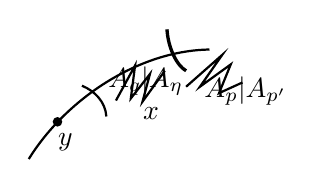
\begin{tikzpicture}[x=1.35cm,y=1.35cm]
  \draw[line width=.8pt] (0,0) .. controls (.34,.55) and (1.02,1.02) .. (1.70,1.03);
  \fill (.27,.35) circle (.045);
  \node[below right,inner sep=0pt] at (.27,.24) {$y$};
  \draw[thick] (.50,.69) .. controls (.62,.64) and (.72,.54) .. (.73,.40);
  \draw[very thick] (1.30,1.22) .. controls (1.31,1.05) and (1.39,.88) .. (1.48,.83);
  \node[inner sep=0pt] at (1.15,.43) {$x$};
  \node[inner sep=0pt] at (1.10,.73) {$\deleted{\unsure{A_q|A_{\eta}}}$};
  \node[inner sep=0pt] at (2.04,.64) {$\deleted{\unsure{A_p|A_{p'}}}$};
  \draw[thick] (.82,.55)--(1.00,.88)--(.96,.57)--(1.14,.80)--(1.07,.54)--(1.28,.83)
    (1.48,.68)--(1.82,.98)--(1.61,.68)--(1.90,.89)--(1.79,.62)--(2.01,.72);
\end{tikzpicture}}

On est amené à prouver le résultat plus fort (remplaçant $A$ par l'anneau $A_f$ d'un voisinage de $y$, pour lequel la condition d'injectivité \unsure{sera|reste|soit} donc \unsure{satisfaite|satisfait}): si $f,g:\operatorname{Spec}(A)\longrightarrow Y$ sont deux morphismes, dont les composés avec $\operatorname{Spec}(A_p)\unsure{-|\to}\operatorname{Spec}(A)$ sont identiques, ils sont identiques.

\uline{Corollaire 3} Supposons que $X$ soit loc. noeth, $Y$ \unsure{loc.} de type fini sur $S$, $S$ loc noeth (ce dernier pt est-il nécessaire ?). La donnée d'un $S$-morphisme équivaut alors à la donnée d'un $S$-hom de $\unsure{\rho|P|p}(\unsure{x|X})$ dans $\rho(Y)$

\uline{\unsure{Remarques|Remarque}} Dans la proposition plus haut\inserted{(et \unsure{$\overline{\mathrm m}$|même} le cor. 1 \unsure{modifié|modulé|seulement})}, la condition imposée à $\unsure{S|F}$ n'est pas \unsure{surabondante}.

Ex. $X=\operatorname{Spec}k[T]$ ($k$ alg. clos], \deleted{\unsure{pour}} \deleted{\unsure{toute|t.}} \deleted{partie} \inserted{\unsure{un|une|ens}} \unsure{finie|fini} $\Phi$ \deleted{de $X-\unsure{a|g|\eta}$ ($a=$ pt gén.).} \inserted{de pts fermés de $X$} on considère \deleted{$F_\Phi=\unsure{0|\coprod}\coprod_{x\in\Phi}\unsure{\varepsilon|\mathcal E|E}_x$, \unsure{soit} $F=\lim F_\Phi$}

$F=\coprod_{x\in X}\varepsilon_x$. On a donc $F_a=e$ ($a$ pt générique) Soit $\xi_x\in\Gamma(\varepsilon_x)$ l'\unsure{élmt|élmt.} \deleted{unité} \inserted{``unité''} de $\Gamma(\varepsilon_x)$, et $\xi_a=e$. Les $\xi_x$ ($x\in X$) forment un syst. cohérent qui \unsure{n'est|n'en} \unsure{pas} une section.
% archive sheet number: 6
